\chapter{Konzept}

Die Konzeption beschäftigt sich zunächst mit einem Überblick des ganzen Prozesses, von der Feature-Extraktion über die Komprimierung bis hin zur Gruppierung. Anschließend folgt eine nähere Betrachtung dieser drei wesentlichen Bestandteile und wie sie ineinander greifen.\newline
Im Kapitel Feature Extraktion werden die Feature-Deskriptoren vorgestellt, die hier verwendet werden: Zum einen der SIFT-Deskriptor, da dieser, neben guten praktischen Resultaten, bereits einigermaßen kompakt ist und auch direkt für die Komprimierung verwendet werden kann. Zum anderen wird ein Feature-Vektor konstruiert, der wesentlichen mehr Komponenten umfasst und sich für den Einsatz der Komprimierung eignet.\newline
Im folgenden Kapitel Autoencoder wird auf der Basis der Arbeit von Zhao \cite{aed2016} ein Stacked Denoising Autoencoder eingeführt, der aus einem Feature-Vektor mit 3042 Komponenten, eine Darstellung des Features in einem Raum mit 36 Dimensionen lernt. Es wird aufgezeigt, wie sich solch ein neuronales Netzwerk mit dem Deep-Learning Framework TensorFlow realisiert werden kann.\newline
Im letzten Kapitel wird das Bag of Visual Words Modell näher betrachtet: Es werden auf Basis der Analyse parallele Varianten des Clustering- und Histogramm-Algorithmus entworfen, die sich zur Ausführung auf Grafikkarten eignen, die CUDA unterstützen. Abschließend wird behandelt, wie der Bag of Visual Words verwendet werden kann, um ein Modell zu generieren bzw. ein Bild zu bewerten.

\section{Modell}

In der Analyse wurden die wesentlichen Bestandteile identifiziert, welche hier zur Gruppierung von Bildern dienen sollen. Im ersten Schritt werden aus den Bildern Features extrahiert und komprimiert, sodass im zweiten Schritt eine Gruppierung der Features in $k$ Gruppen erfolgen kann.
Der erste Schritt lässt sich wieder in zwei Phasen unterteilen, von denen die Zweite, je nach Feature-Detektor / -Deskriptor, optional ist:

\begin{itemize}
	\item \textbf{Extraktion der Features} Zuerst muss das Verfahren bestimmt werden, mit denen die Features gewonnen werden sollen. Je nach Anwendungsfall sollte dieses Verfahren austauschbar sein. Als Ergebnis wird ein Feature-Vektor zurückgegeben. Dieser Vektor enthält Komponenten normalisiert im Intervall zwischen 0 und 1, die abhängig vom Verfahren verschiedene Eigenschaften beschreiben.
	\item \textbf{Komprimierung der Features} Um die Komponenten in einem Feature-Vektor auf die Wesentlichen zu reduzieren, erfolgt eine Komprimierung durch einen Autoencoder. Als Ergebnis wird wieder ein Feature-Vektor zurückgegeben, der weniger Komponenten enthält. Sollte der verwendete Feature-Vektor bereits kompakt genug sein, ist diese Phase nicht notwendig. 
\end{itemize} 

\begin{figure}
	\centering
	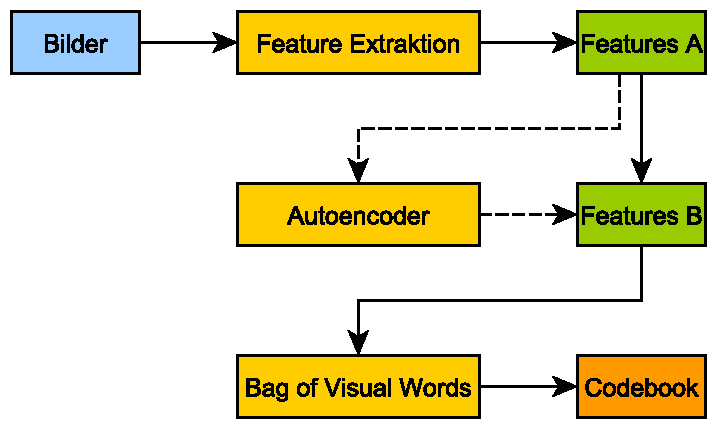
\includegraphics[scale=0.85]{images/model.pdf}
	\caption{Aufbau des Modells}
	\label{img:model}
\end{figure}

In Abbildung \ref{img:model} ist das Modell im Ganzen dargestellt.  Jede \glqq Zeile \grqq  entspricht hier einer Phase der Verarbeitung. Diese Phasen werden im Folgenden detailliert dargestellt, hier soll jedoch zuerst ein Überblick über den Ablauf gegeben werden. Zu Beginn werden aus den Bilddaten \textit{Images} durch einen Feature-Extraktor die Feature-Vektoren \textit{Features A} erhoben. Die Phase des Autoencoders ist hierbei optional und daher gestrichelt dargestellt. Sollten die Features nicht durch den Autoencoder komprimiert werden, sind diese gleich der Menge \textit{Features B}, die sonst vom Autoencoder erzeugt wird. In der dritten Phase nimmt der Bag of Visual Words die Features aus der vorigen Phase entgegen und generiert hieraus das \textit{Codebook}.\newline

\section{Feature Extraktion}

Da es zahlreiche Verfahren zur Detektion und Extraktion von Features aus Bildern in Literatur und Praxis gibt, können diese unmöglich alle gleichermaßen Beachtung finden. In der Analyse wurde bereits auch diskutiert, dass über die Daten der HsH keine Annahmen getroffen werden können. Gegenstand dieser Arbeit soll daher die Objekterkennung im Bildern sein. Für diesen Zweck sollen im Weiteren zwei Deskriptoren ausgewählt werden:

\begin{itemize}
	\item Da die Schritte im Prozess aufeinander aufbauen, hängt die Qualität der Ergebnisse des Bag of Visual Word Verfahrens auch vom Autoencoder ab. Um den Bag of Visual Words an sich testen zu können, soll ein bereits kompakter, praktisch bewährter Deskriptor als Alternative dienen.
	\item Es ist denkbar, dass der Schritt der Komprimierung nicht in allen Fällen notwendig bzw. sinnvoll ist, da der Deskriptor bereits kompakt genug ist.
\end{itemize} 

Viele Verfahren erzeugen bereits einen kompakten Deskriptor. Beispielsweise ist die Komprimierung eines SIFT-Deskriptors (128 Komponenten) wahrscheinlich wenig erfolgreich: Der Autoencoder müsste 128 Neuronen im \textit{input layer} besitzen. Zur Komprimierung bleibt dann wenig \glqq Platz\grqq  im Netz, es sei denn es werden mehrere \textit{hidden layer} verwendet, deren Neuronenanzahl zunächst ansteigt. Ziel soll es hier aber sein einen Deskriptor zu erzeugen der zu Anfang viele Komponenten aufweist, um so einen Stacked Autoencoder zu trainieren, der mit jeder Schicht einen kompakteren Deskriptor liefert. Auf diese Weise können auch zum Experimentieren mehrere Deskriptoren generiert werden, deren Form von Anzahl der \textit{hidden layer} und deren Neuronenanzahl abhängt.\newline
Zhao \cite{aed2016} hat aus diesem Grund einen Feature-Vektor mit $3042$ erzeugt, der dann anschließend durch einen Autoencoder komprimiert wird. Die \textit{keypoints} werden hier durch den SIFT-Detektor ermittelt. Um jeden der \textit{keypoints} wird eine Nachbarschaft der Größe $41 \times 41$ betrachtet. Von diesen Ausschnitten werden die Gradienten in horizontale und vertikale Richtung bestimmt. Bei einem Einsatz eines Gauß- oder Sobelfilters mit einer Filterkerngröße von $3 \times 3$, ergeben sich somit pro Richtung $1521$ Werte, die den Ausschnitt beschreiben. Der resultierende Feature-Vektor besitzt somit, für beide Richtungen, insgesamt $3042$ Komponenten.
\todo{SIFT Alternative}

\section{Autoencoder}

In diesem Ansatz wird ein Stacked Denoising Autoencoder zur Komprimierung eines Feature-Vektors entworfen, wie er in der Arbeit von Zhao \cite{aed2016} vorgeschlagen wurde. In einem Experiment wurde gezeigt, dass dieser Autoencoder \textit{state of the art} Ergebnisse erzielt: die Ergebnisse wurden unter verschiedenen Kriterien mit denen der Hauptkomponentenanalyse (PCA) und SIFT-PCA verglichen. Dabei erkannte der Autoencoder in fast allen die gleichen Features, jedoch durch einen 36 statt 128-elementigen Feature-Vektor. Aus diesem Grund soll Zhaos Autoencoder adaptiert werden. \newline
Es wird zunächst auf den Aufbau des Netzes eingegangen: Anzahl der Schichten sowie der Neuronen, Aktivierungsfunktionen und weitere Parameter des Netzes. Abschließend werden der Trainings- und Testprozess beschrieben, so wie sie von Zhao ausgeführt wurden.

\subsection{Modell und Parameter}

\todo{Lernrate etc.} Der Encoder des vorgeschlagenen Modells besteht aus fünf Schichten, deren Neuronenanzahl sukzessive reduziert wird, bis schließlich die kleinste Schicht mit 36 Neuronen erreicht wird. Abbildung \ref{img:ae_model} zeigt die Schichten des Encoders sowie Decoders. Der Decoder ist umgekehrt aufgebaut und auch die Gewichte der Kanten zwischen zwei Neuronen entsprechen ihren Pendants im Encoder.

\begin{figure}
	\centering
	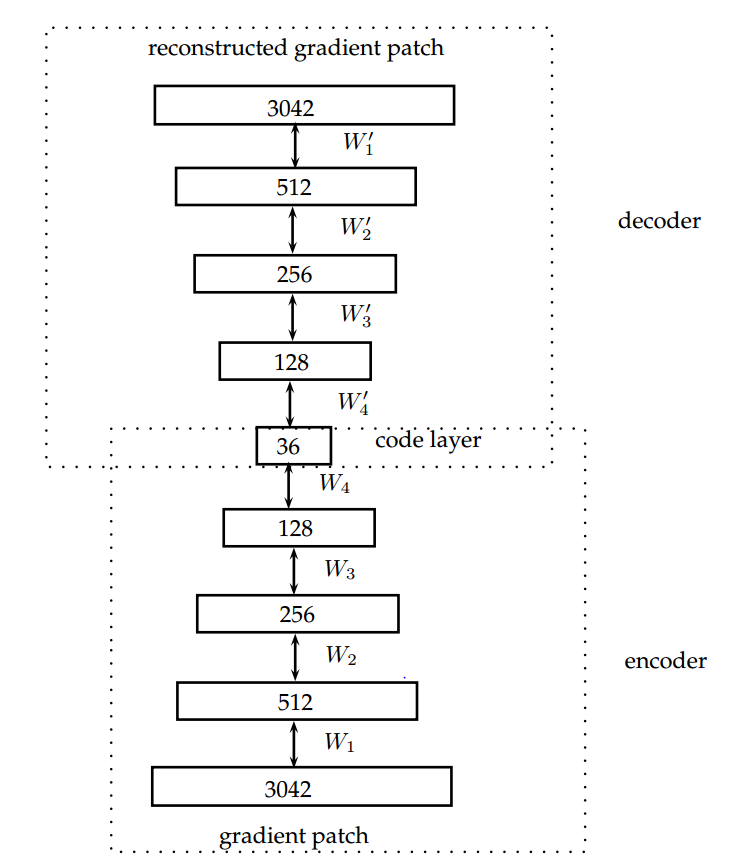
\includegraphics[scale=0.6]{images/ae_model.png}
	\caption{Schichten des verwendeten Autoencoders \cite{aed2016}}
	\label{img:ae_model}
\end{figure}

Die Hyperparameter für das verwendete Modell sind auch vollständig dokumentiert. Zhao verwendete hier folgende Werte:

\begin{itemize}
	\item Lernrate: $l = 0.02$
	\item Trainingsiterationen: $t_i =$ Iterationen der i-ten Schicht \newline
	  $t_1$:       $1000$\newline
	  $t_2$:       $ 700$\newline
	  $t_{3,4,5}$: $ 500$
	\item Batch size: $B = 128$
\end{itemize}

\subsection{TensorFlow}

TensorFlow ist ein Deep-Learning Framework, dass in Python geschrieben ist. Darüber hinaus gibt aus aber auch Schnittstellen zu anderen Sprachen wie beispielsweise C oder Java. Aus dem Namen leitet sich die bereits die Idee ab, die TensorFlow zugrunde liegt: Ein Tensor ist ein (multidimensionales) Array aus Daten. Diese Tensoren sind mit mathematischen Operationen, den Knoten, miteinander verbunden, sodass die Daten durch die Tensoren und Knoten \grqq fließen\grqq und dabei transformiert werden. Daher eignet sich TensorFlow hervorragend für die Darstellung neuronaler Netze: Die Kanten des Netzes entsprechen den Tensoren, die Neuronen in den Schichten führen mathematische Operationen auf den eingehenden Daten aus und leiten diese weiter an den nächsten Tensor. Die in TensorFlow definierten Modelle lassen sich sowohl auf mehreren CPUs sowie Nvidia GPUs ausführen. Hierfür ist es notwendig, dass auf dem System mindestens CUDA $7.5$ und die cuDNN Bibliothek $4.0$ installiert ist. 
TensorFlow folgt dem sogenannten \glqq lazy\grqq  Programmierparadigma. Dies bedeutet, dass zunächst aus den Definitionen ein Modell aufgebaut wird. Dieses Modell kann durch TensorFlow automatisiert geprüft und visualisiert werden. Im nächsten Schritt werden alle nötigen Variablen initialisiert. Erst durch das Erzeugen und Aufrufen einer \glqq Session\grqq wird das Modell trainiert bzw. auf Testdaten ausgeführt.

\lstset{language=Python}
\begin{lstlisting}
import tensorflow as tf

a = tf.placeholder(tf.int16)
b = tf.placeholder(tf.int16)

addOp = tf.add(a, b)

init = tf.initialize_all_variables()

with tf.Session() as sess:
    sess.run(init)
    print "Addition: %i" % sess.run(addOp, feed_dict={a: 2, b: 3})

sess.close()
\end{lstlisting}

\section{Bag of Visual Words}

In der Analyse wurde bereits sequentielle Varianten des Lloyd und Histogramm Algorithmus vorgestellt und aufgezeigt, an welchen Stellen eine Parallelisierung der Berechnung durch Grafikkarten erfolgen kann. Im Folgenden wird aus diesen Informationen je Algorithmus eine parallele Version abgeleitet, welche sich für die Realisierung als CUDA Programm eignen.
Im Abschnitt Modell wird dann der Aufbau des Modells und Ablauf der Funktionsaufrufe skizziert. Zur Interaktion stehen einem Anwender im Wesentlichen eine Funktion zu Generierung eines Modells und zur Berechnung der \textit{Visual Words} eines Bildes zur Verfügung.

\subsection{Parellisierung von Llyods Algorithmus}

Der Thread in einem Block mit der \textit{threadId} 0 fungiert hier als Master für die anderen Threads. Die Initialisierung der Cluster mit zufälligen Vektoren aus $v$ wird ebenfalls von diesem übernommen. Die Zuweisung von Vektoren zu Clustern nimmt $\Theta(nk)$ Zeit in Anspruch, wobei $n$ die Anzahl Vektoren und $k$ die Anzahl der Cluster ist. Diese Phase kann parallelisiert werden, in dem pro Feature Vektor ein Thread verwendet wird: Jeder Thread berechnet für seinen Feature Vektor die Distanz zu allen Clusterschwerpunkten und bestimmt den Index des Clusters, der am Nächsten ist. Dieser Prozess ist in Pseudocode in Zeile 6 bis 8 ausgedrückt. Bevor die Cluster aktualisiert werden, müssen die Threads synchronisiert werden: Andernfalls ist nicht garantiert, dass die Berechnung jedes Threads abgeschlossen ist.

\lstset{language=C}
\begin{lstlisting}[mathescape=true]
kmeans_gpu
	if threadId == 0
		$c_{j} = rand(p_{i}) \in P, \: j = 1,...,k, \: c_{j} \neq c_{i} \: \forall i \neq j$
	synchronize threads
	until convergence
		for each $x_{i} \in P_{threadId}$
			$l_{i} = argminD(c_{j}, p_{i})$
		synchronize threads
		if threadId == 0
			for each $p_{i} \in P$
				$c_{l_{i}} = c_{l_{i}} + p_{i}$
				$m_{l_{i}} = m_{l_{i}} + 1$
			for each $c_{j} \in C$
				$c_{j} = \frac{1}{m_{j}} c_{i}$
\end{lstlisting}

\subsection{Parallele Reduzierung von Histogrammen}

Die Berechnung eines Histogramms kann parallelisiert werden, da die Operation assoziativ und kommutativ ist: Es spielt keine Rolle in welcher Reihenfolge die Daten abgearbeitet werden bzw. in welcher Reihenfolge die Klassen inkrementiert werden. Wenn das zu beschreibende Histogramm im \textit{global memory} vorliegt, wird die Berechnungsgeschwindigkeit stark reduziert, da viele Threads auf die gleichen Speicheradressen des Histogramms schreibend zugreifen. Damit es nicht zu Lese- / Schreibanomalien kommt, muss das Inkrementieren einer Klasse atomar sein, d.h. zwischen Lese- und Schreibzugriff darf kein anderer Thread auf die Adresse zugreifen. Dies wird in CUDA durch die Operation \textit{atomicAdd} realisiert. Damit die Anzahl an Threads die auf dieselbe Adresse schreiben eingeschränkt wird, arbeitet jeder Block auf einem lokalen Histogramm im \textit{shared memory}. Wenn alle Blöcke ihre lokalen Histogramme berechnet haben, müssen diese noch in das Histogramm im \textit{global memory} kumuliert werden.

\lstset{language=C}
\begin{lstlisting}
__global__
void histogram_kernel (float *buffer, long size, int *histo, int bins) {
	extern __shared__ int *copy[];
	
	if (threadIdx.x < bins) {
		copy[threadIdx.x] = 0;		
	}
	__syncthreads();

	int id = threadIdx.x + blockDim.x * gridDim.x;
	int stride = blockDim.x * gridDim.x;
	
	while (i < stride) {
		int bin = buffer[i] / bins; 
		atomicAdd(&(copy[bin]), 1);
		i += stride;	
	}
	__syncthreads();
	
	if (threadIdx.x < bins) {
		atomicAdd(&(histo[threadIdx.x]), copy[threadIdx.x]);		
	}
}
\end{lstlisting} 

\subsection{Aufbau des Bag of Visual Words Algorithmus}

Das Bag of Visual Words Modell soll zwei Anwendungsfälle unterstützen. Zunächst muss aus einer Menge von Bildern ein Modell generiert werden. Um Modelle über den Speicher hinaus verwenden zu können, soll die Funktion angeboten werden, diese persistent zu speichern bzw. wieder einzulesen. Der Abschnitt Generierung des Modells beschäftigt sich mit einem Entwurf solch eines Systems. Sofern ein Modell generiert wurde, soll es möglich sein, dass Histogramm der \textit{Visual Words} weiterer Bilder zu bestimmen. Auf diese Weise können Ähnlichkeiten zwischen Bildern auf Basis ihrer Histogrammdarstellung gemessen werden. Dieser Prozess ist in Kapitel Labeling eines Bildes dargestellt.

\subsubsection{Generierung des Modells}

Die Generierung eines Modells kann durch die Funktion \textit{generateModel} gestartet werden. Als Parameter werden der Pfad für die Bilddaten \textit{imageDir}, der Zielpfad \textit{modelPath} und die Anzahl der Cluster \textit{k} erwartet. Der Ablauf der folgenden Funktionsaufrufe ist in Abbildung \ref{img:concept_bovw_1} dargestellt. Im ersten Schritt wird \textit{extractFeatures} aufgerufen, um alle SIFT Features der Bilder, die in \textit{imageDir} enthalten sind, zu extrahieren. Als nächstes werden durch \textit{clusterFeatures} die Features in \textit{k} Cluster gruppiert. Die Berechnung der Cluster, der Distanzen von Features zu Clustern und des Konvergenzkriteriums erfolgt durch die GPU. Als Ergebnis werden die $k$ berechneten Schwerpunkte der Cluster und die Mitgliedschaft der Features zurückgegeben. Abschließend speichert \textit{saveModel} die Cluster unter dem Pfad  \textit{modelPath}/clusters und die Mitgliedschaft unter \textit{modelpath}/membership. \todo{single extractFeature}

\begin{figure}
	\centering
	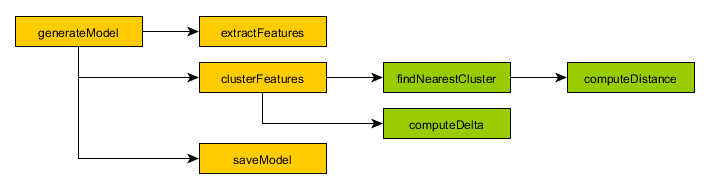
\includegraphics[scale=0.8]{images/concept_bovw_1.png}
	\caption{Funktionen zur Generierung eines Modells}
	\label{img:concept_bovw_1}
\end{figure}

\subsubsection{Vergleich von Bildern}

Sofern ein Modell erstellt wurde, können auf dessen Basis Bilder, bzw. deren Features, verglichen werden. In Abbildung \ref{img:concept_bovw_2} sind schematisch die aufeinanderfolgenden Funktionsaufrufe dargestellt. Die Funktion \textit{compareImages} erwartet als Argumente die Pfade zu den Bildern. Es wird von beiden Bildern das Histogramm der Visual Words durch \textit{computeVisualWords} berechnet. Hier wird auf der GPU die parallele Reduzierung der Histogramme durchgeführt. Anschließend wird der Fehler, hier als MSE gemessen, berechnet und die Ähnlichkeit als $1 - MSE$ zurückgegeben. Liegen nun zwei Bildern in der gleichen Kategorie, sollte sich ihre Histogrammdarstellung bei adäquatem $k$ ähneln. 

\begin{figure}
	\centering
	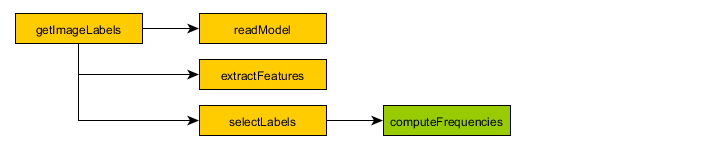
\includegraphics[scale=0.8]{images/concept_bovw_2.png}
	\caption{\todo{NEU}}
	\label{img:concept_bovw_2}
\end{figure}

